\chapter{Introduction}
\label{cha:intro}

%\cleanchapterquote{You can’t do better design with a computer, but you can speed up your work enormously.}{Wim Crouwel}{(Graphic designer and typographer)}


\section{Motivation}
\label{sec:intro:motivation}

All cells in an organism have the same genetic information and are still able to execute very different functions.

\section{Biological Background}
\label{sec:intro:bio}

\begin{figure}[h]
	\centering
	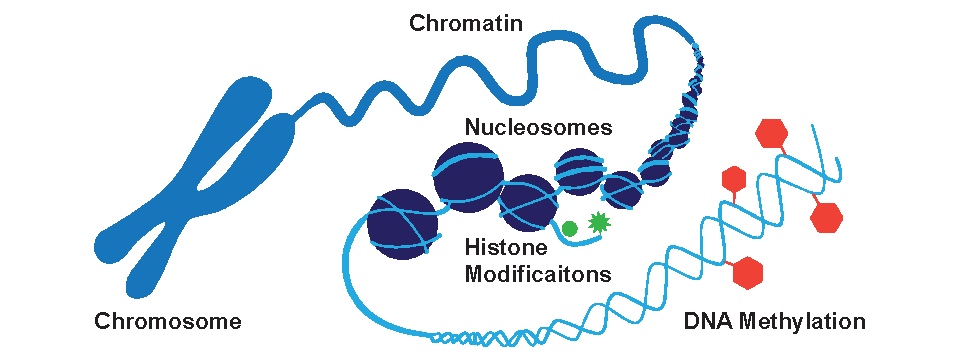
\includegraphics[width=1.0\textwidth]{figures/intro/chromatin.pdf}
	\captionsetup{format=plain}
	\caption[Structure]{Chromosome to nucleotide structure (Adapted from \cite{zymo2020})}
	\label{fig:intro:chromatin}
\end{figure}

\begin{figure}[h]
	\centering
	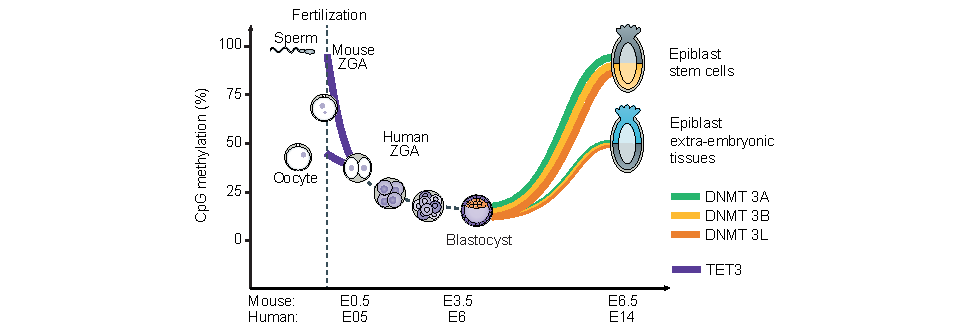
\includegraphics[width=1.0\textwidth]{figures/intro/methylation.pdf}
	\captionsetup{format=plain}
	\caption[DNA methylation dynamics]{Methylation dynamics during development (Adapted from \cite{Greenberg2019})}
	\label{fig:intro:methylation}
\end{figure}

\begin{itemize}
    \item Organism, cell, DNA
    \item Epigenetics as additional layer
    \begin{itemize}
        \item Briefly histone modifications
        \item DNA methylation, 5mC, hmC, 6mA
    \end{itemize}
    \item Without explicit statement: Focus of the Meissner lab
\end{itemize}


\section{Technical Background}
\label{sec:intro:sequencing}

\begin{figure}[h]
	\centering
	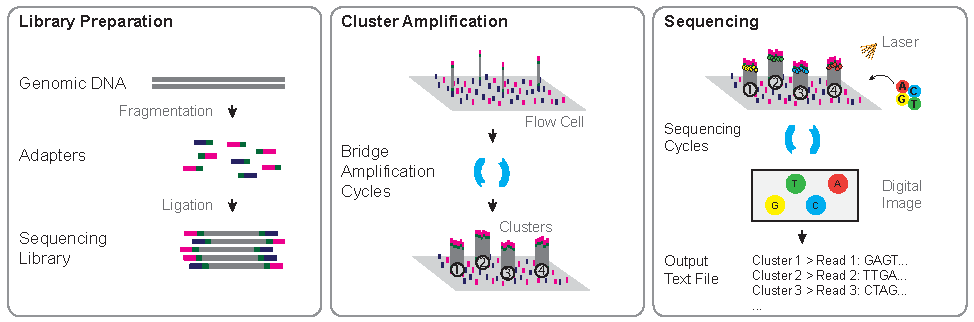
\includegraphics[width=1.0\textwidth]{figures/intro/sbs.pdf}
	\captionsetup{format=plain}
	\caption[Sequencing by synthesis]{Sequencing by synthesis}
	\label{fig:intro:sbs}
\end{figure}

\begin{figure}[h]
	\centering
	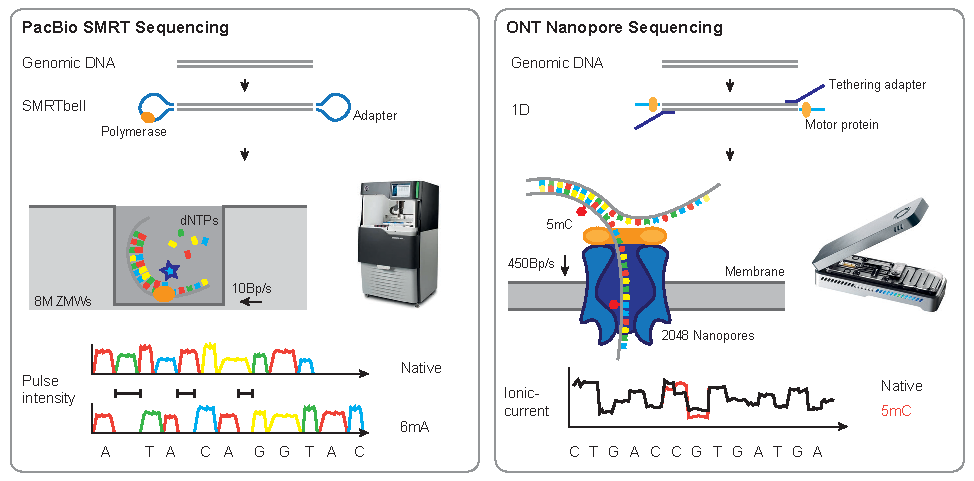
\includegraphics[width=1.0\textwidth]{figures/intro/long_read.pdf}
	\captionsetup{format=plain}
	\caption[Long read sequencing]{PacBio SMRT and ONT nanopore sequencing.}
	\label{fig:intro:longread}
\end{figure}

\begin{itemize}
    \item Sequencing
    \item Helene: "Easy to forget: but how to calculate a methylation rate from multiple reads and why minimum coverage. There is even a ref for 10X."
    \item Breifly generations, 1st, 2nd, 3rd ...
    \item Detail 3rd generation
    \begin{itemize}
        \item Briefly PacBio, Roche
        \item Detail ONT
    \end{itemize}
\end{itemize}

Third-generation sequencing techniques are currently introducing new perspectives to the field of genome analysis by generating previously unattainable read lengths with averages in the tens of thousands of nucleotides. Among other devices distributed by Oxford Nanopore Technologies (ONT), the MinION in particular is gaining prominence. In brief, the nanopore sequencing process is based on guiding a nucleotide polymer through a pore inserted in a membrane while measuring a change in ionic current as a proxy signal over time. This signal is then interpreted to determine the underlying DNA or RNA sequence. The nanopore technology enables direct readout of sequences from individual DNA or RNA molecules, including base modifications, since no synthesis or amplification is required.

\section{Structure}
\label{sec:intro:structure}

Briefly describe the overall structure of the thesis, from literature to pipeline, signal processing and finally repeat detection.

%\textbf{Chapter \ref{sec:nanopype}} \\[0.2em]
%\blindtext

